%% LaTeX-Beamer template for KIT design
%% by Erik Burger, Christian Hammer
%% title picture by Klaus Krogmann
%%
%% version 2.1
%%
%% mostly compatible to KIT corporate design v2.0
%% http://intranet.kit.edu/gestaltungsrichtlinien.php
%%
%% Problems, bugs and comments to
%% burger@kit.edu

\documentclass[18pt]{beamer}
\usepackage[utf8]{inputenc}
%% SLIDE FORMAT

% use 'beamerthemekit' for standard 4:3 ratio
% for widescreen slides (16:9), use 'beamerthemekitwide'

\usepackage{templates/beamerthemekit}
% \usepackage{templates/beamerthemekitwide}

%% TITLE PICTURE

% if a custom picture is to be used on the title page, copy it into the 'logos'
% directory, in the line below, replace 'mypicture' with the 
% filename (without extension) and uncomment the following line
% (picture proportions: 63 : 20 for standard, 169 : 40 for wide
% *.eps format if you use latex+dvips+ps2pdf, 
% *.jpg/*.png/*.pdf if you use pdflatex)

%\titleimage{mypicture}

%% TITLE LOGO

% for a custom logo on the front page, copy your file into the 'logos'
% directory, insert the filename in the line below and uncomment it

\titlelogo{banner.jpg}

% (*.eps format if you use latex+dvips+ps2pdf,
% *.jpg/*.png/*.pdf if you use pdflatex)

%% TikZ INTEGRATION

% use these packages for PCM symbols and UML classes
% \usepackage{templates/tikzkit}
% \usepackage{templates/tikzuml}

% the presentation starts here

\title[Geometrie 2]{Geometrie 2 - ICPC Praktikum SS14}


\institute{Tobias Hornberger $\cdot$ Paul Jungeblut $\cdot$ Enja Stein $\cdot$ Lena Winter}

\begin{document}

% change the following line to "ngerman" for German style date and logos
\selectlanguage{ngerman}

%title page
\begin{frame}
\titlepage
\end{frame}

\section{Konvexe Hülle}
	\subsection{Problemstellung}
		\begin{frame}{Problemstellung: Konvexe Hülle}
			\begin{block}{Problem}
			 Gegeben sei eine Menge M von Punkten in der Ebene. Die konvexe Hülle von M ist die kleinste konvexe Menge, in der M enthalten ist.
			\end{block}
			\begin{figure}
				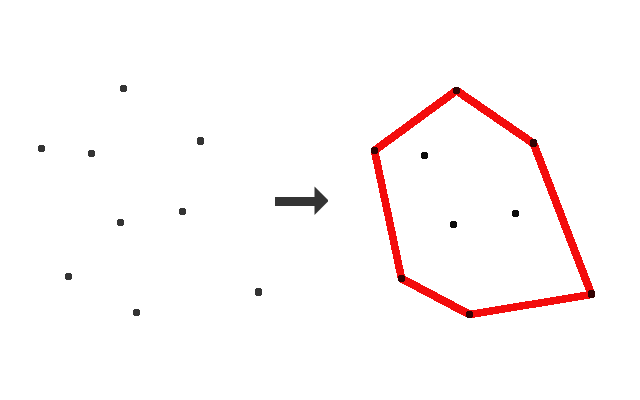
\includegraphics[width=8cm]{logos/konhu.png}\\
			\end{figure}
		\end{frame}
		
	\subsection{Idee}
		\begin{frame}{Hüllen}
			\begin{minipage}[t]{0.45\textwidth}
				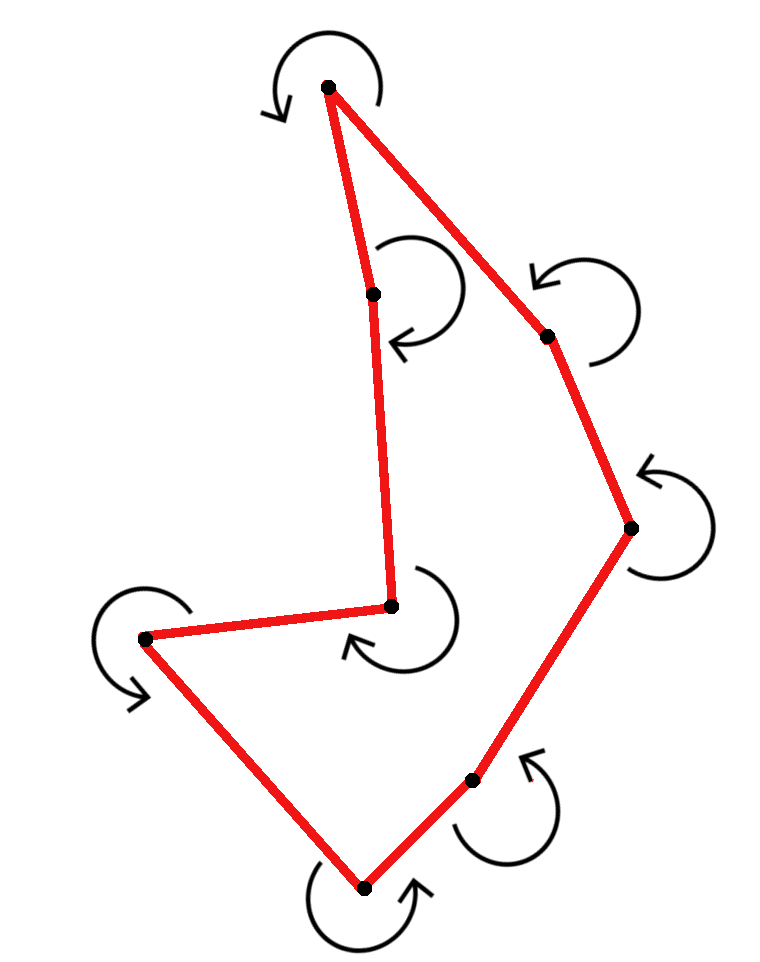
\includegraphics[width=0.8\textwidth]{logos/nKonvex.png}
			\end{minipage}
			\begin{minipage}[t]{0.45\textwidth}
				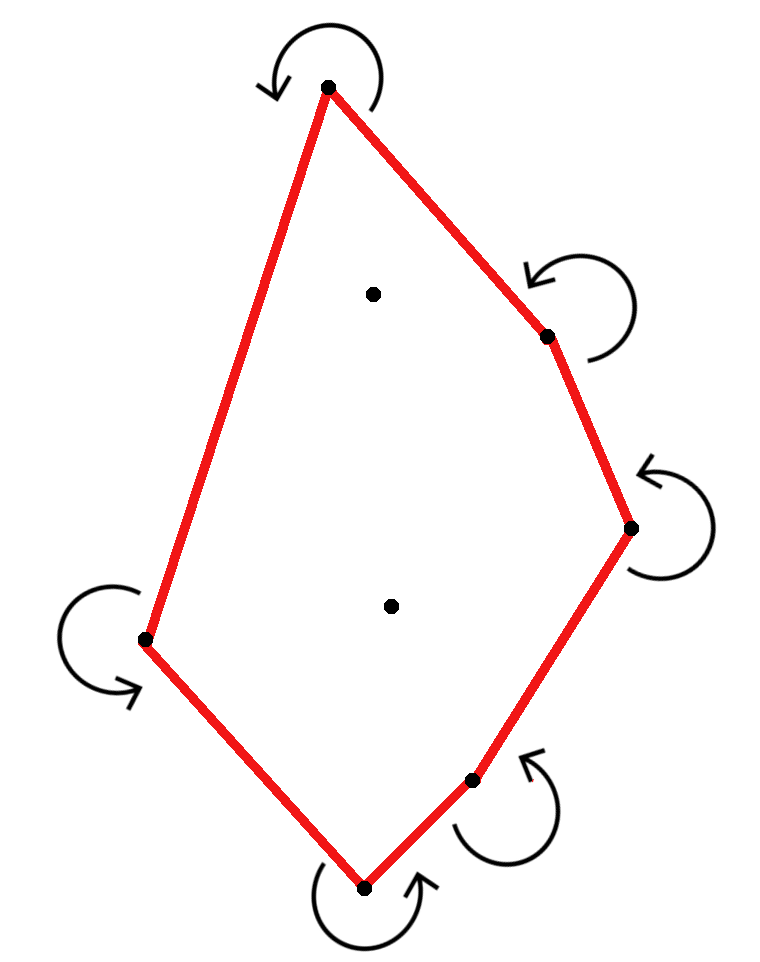
\includegraphics[width=0.8\textwidth]{logos/konvex.png}
			\end{minipage}
			\begin{block}{Fazit}
				Konvexe Hüllen haben nur links Abbiegungen.
			\end{block}
		
		\end{frame}
	
	\subsection{Graham Scan}
		\begin{frame}{Idee: Graham Scan}
			\begin{itemize}
				\item Bestimme den untersten Punkt $ P_0 $
				\item Sortiere die Punkte nach Winkel relativ zu $ P_0 $
				\item Füge den Punkt mit dem größten Winkel der konvexen Hülle hinzu
				\item Nimm nun jeweils den Punkt mit dem kleinsten Winkel und überprüfe mit CCW:
				\begin{itemize}
					\item liegt er links des Vektors $P_{k-1}$ $P_k$ füge ihn der konvexen Hülle hinzu
					\item liegt er rechts so entferne solange Punkte aus der Konvexen Hülle bis er links des letzten Vektors liegt 
				\end{itemize}
				\item Wurden alle Punkte betrachtet so hat man die konvexe Hülle gefunden.
			\end{itemize}
		\end{frame}
		
		\begin{frame}{Idee: Graham Scan}
			\begin{block}{Sonderfälle}
				\begin{itemize}
					\item Liegen drei Punkte auf einer Linie wird das als Linksknick interpretiert
					\item Haben zwei Punkte den gleichen Winkel so werden Sie lexikographisch sortiert.
				\end{itemize}
			\end{block}
		\end{frame}
		
		
		\begin{frame}{Beispiel}
		\begin{minipage}[t]{\textwidth}
		\begin{center}
			\includegraphics<1>[width=0.5\textwidth]{logos/winkel.png}
			\includegraphics<2>[width=0.5\textwidth]{logos/pf1.png}
			\includegraphics<3>[width=0.5\textwidth]{logos/pf2.png}
			\includegraphics<4>[width=0.5\textwidth]{logos/pf3.png}
			\includegraphics<5>[width=0.5\textwidth]{logos/pf4.png}
			\includegraphics<6>[width=0.5\textwidth]{logos/pf45.png}			
			\includegraphics<7>[width=0.5\textwidth]{logos/pf5.png}
			\includegraphics<8>[width=0.5\textwidth]{logos/pf67.png}
			\includegraphics<9>[width=0.5\textwidth]{logos/pf677.png}
			\includegraphics<10>[width=0.5\textwidth]{logos/pf6.png}
		\end{center}
		\end{minipage}
		\end{frame}
	


\section{Sweepline}
\begin{frame}{Sweepline - Was ist das?}
	\begin{block}{Sweepline} 
		\begin{itemize}
			\item Häufige Methode zum Lösen geometrischer Probleme
			\item Gesamte Ebene wird mit einer Linie gescannt (Scanline)
			\item Nur an bestimmten, wichtigen Punkten (Events) muss etwas getan werden
		\end{itemize}
	\end{block}
	\begin{exampleblock}{Beispiele}
		\begin{itemize}
			\item Graham-Scan, Sweepline scannt um einen Punkt rotierend
			\item Closest-Pair, klassisch
		\end{itemize}
	\end{exampleblock}
\end{frame}

\subsection{Problem}
\begin{frame}{Problemstellung}
	\begin{block}{Aufgabe}
		\begin{itemize}
			\item $n$ Strecken in der Ebene, jeweils gegeben durch die beiden Endpunkte
			\item \textbf{Aufgabe:} Finde alle Schnittpunkte
		\end{itemize}
	\end{block}
	
	\begin{block}{Vereinfachungen}
		\begin{itemize}
			\item keine zwei End-/Schnittpunkte haben die gleiche x-Koordinate
			\item kein Endpunkt liegt auf einer anderen Strecke
			\item max. 2 Strecken schneiden sich in einem Punkt
		\end{itemize}
	\end{block}
\end{frame}

\begin{frame}{Naiver Ansatz}
	\begin{exampleblock}{Erinnerung}
		$Schnitt(p_1, p_2, p_3, p_4) = \newline
		\hspace*{1cm} ccw(p_1, p_2, p_3) \cdot ccw(p_1, p_2, p_4) \le 0 \wedge \newline
		\hspace*{1cm} ccw(p_3, p_4, p_1) \cdot ccw(p_3, p_4, p_2) \le 0$\newline
		\\ 
	\end{exampleblock}
	\begin{flushright}
	\begin{figure}
		\vspace{-2.5cm}\hspace*{6cm}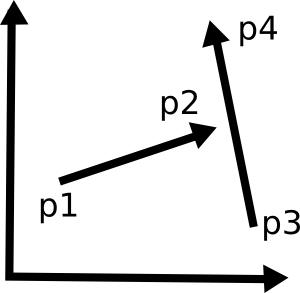
\includegraphics[width=2cm]{logos/intersect.png}\\
	\end{figure}
	\end{flushright}
	\hspace{3cm}
	\begin{block}{Algorithmus}
		\begin{itemize}
			\item Teste für je zwei Strecken, ob sie sich schneiden
			\item Berechne Schnittpunkt (LGS)
			\item Laufzeit: $O\left(n^2\right)$
		\end{itemize}
	\end{block}
\end{frame}

\begin{frame}{Bentley–Ottmann Algorithmus}
	\begin{block}{Idee}
		\begin{itemize}
			\item Lasse Sweepline $L$ von links nach rechts über die Ebene laufen.
			\item Zu jedem Zeitpunkt schneidet S eine Teilmenge der Strecken. Die vertikale Anordnung verändert sich dabei nur bei einem Schnittpunkt.
			\item Events sind
				\begin{itemize}
					\item noch nicht gescannte Endpunkte
					\item Schnittpunkte von Strecken, die in der vertikalen Anordnung nebeneinander liegen
				\end{itemize}
		\end{itemize}
	\end{block}
\end{frame}

\begin{frame}{Bentley–Ottmann Algorithmus}
	\begin{block}{Algorithmus - Initialisierung}
		\begin{enumerate}
			\item Erstelle Priority Queue $pq$ für zukünftige Events, priorisiert nach x-Koordinate. $pq$ enthält zu Beginn alle Endpunkte.
			\item Erstelle Set $T$ für vertikale Anordnung der Schnittpunkte zwischen den Strecken und der Sweepline. Sortierung nach y-Koordinate. Zu Beginn leer.
		\end{enumerate}
	\end{block}
\end{frame}

\begin{frame}{Bentley–Ottmann Algorithmus}
	\begin{block}{Algorithmus - Fortsetzung}
		\begin{enumerate}
			\setcounter{enumi}{2}
			\item Solange $pq$ nicht leer ist, entferne erstes Element aus $pq$.
			\begin{itemize}
				\item \textbf{Linker Endpunkt einer Strecke $s$:} Füge $s$ in $T$ ein. Suche Strecken $r$ und $t$ direkt über und unter $s$ (falls sie existieren). Falls ihr Schnittpunk als Event in $pq$ liegt, entferne ihn. Falls $s$ die Strecken $r$ oder $t$ schneidet, füge die Schnittpunkte in $pq$ ein.
				
				\item \textbf{Rechter Endpunkt einer Strecke $s$:} Suche Strecken $r$ und $t$ direkt über und unter $s$. Falls sie sich noch schneiden, füge Schnittpunk zu $pq$ hinzu. Entferne $s$ aus $T$. 
				
				\item \textbf{Schnittpunk zweier Strecken $s$, $t$:} Tausche Positionen von $s$ und $t$ in $T$. Finde Strecken $o$ und $u$ darüber und darunter. Entferne Schnittpunkte mit diesen, füge neue ein.
			\end{itemize}
		\end{enumerate}
	\end{block}
\end{frame}

	
\section{Closed Pair}

	\subsection{Problemstellung}
		\begin{frame}{Problemstellung: Closed Pair}
			\textbf{Geben:} n Punkte auf einer Ebene \\
			\textbf{Gesucht:} die beiden am nähesten zusammenliegenden Punkte\\
		
			\begin{block}{Naiver Ansatz}
				Mit Vollständiger Suche. \\
				\ \\
				Alle Distanzen zwischen allen möglichen Punktpaaren ausrechnen und davon das Minimum wählen. 
				\ \\
				\textbf{Laufzeit:} $\mathcal{O}(n^2)$
			\end{block}	
		\end{frame}
	
	\subsection{Divide and Conquer}
		\begin{frame}{Idee: Divide and Conquer}
			Statt Vollständiger Suche: Divide \& Conquer für eine Lösung in $\mathcal{O}(n \log n)$ Zeit.

			\begin{enumerate}
				\item \textbf{Divide}:\\ Sortieren der Punkte (Primär x-Koordinate, sekundär y-Koordinate). Aufteilen der Punktmenge in zwei Hälften
				\item \textbf{Conquer}:\\ Größe der Punktmengen:
					\begin{itemize}
						\item $|$Punktmenge$|$ = 1, return $ \infty$
						\item $|$PunktMenge$|$ = 2, return Euklidische Distanz der beiden Punkte
					\end{itemize}
				\item \textbf{Combine}: \\ Sei $d_{1}$ die kleinste Distanz innerhalb der Punktmenge $A_1$. \\
							Sei $d_2$ die kleinste Distanz innerhalb der Punktmenge $A_2$. \\
							Sei $d_{3}$ die kleinste Distanz von 2 Punkte aus jeweils $A_{1}$ und $A_{2}$.\\
							$\rightarrow$ Die kleinste Distanz innerhalb $A_1$ $\cup$ $A_2$ ist $\min(s_1,s_2, s_3)$ \\
			\end{enumerate}
		\end{frame}

		\begin{frame}{Combine}
			Naiver Ansatz für Combine immer noch in Laufzeit $\mathcal{O}(n^2)$ \\
			\centerline{\huge{Optimierbar!}} \\
			Sei $d' = \min(d_1, d_2)$. \\  
			Für jeden Punkt in der unteren Punktmenge kann der nähere Punkt nur in einem Rechteck mit Breite $d' \text{und Höhe} \ 2 * d'$ liegen
			\begin{block}{Beweisbar}
				Es gibt maximal 6 solche Punkte im Rechteck. \\
				Ohne Beweis
			\end{block}
			\ \\
			$\Rightarrow$ Maximal $\mathcal{O}(6n)$ Operationen für Combine \\
			$\Rightarrow$ \textbf{Gesamtlaufzeit:} \\ $T(n) = 2 * T(n/2) + \mathcal{O}(n)$, und es gilt: $T(n) \in \mathcal{O}(n \log n)$
		\end{frame}

		\begin{frame}{Beispiel}
			\begin{minipage}{0.45\textwidth}
				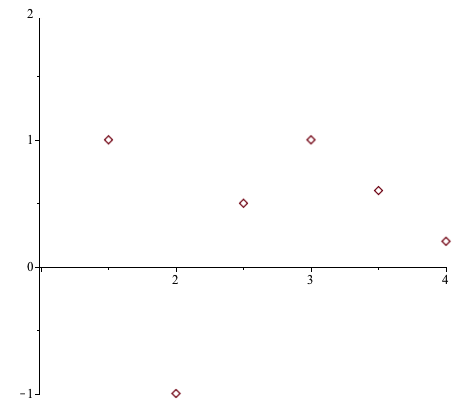
\includegraphics[width =\textwidth]{logos/PlotsBetter.png}
			\end{minipage}
			\begin{minipage}{0.45\textwidth}
				Ausgangslage		
			\end{minipage}
		\end{frame}

		\begin{frame}{Beispiel}
			\begin{minipage}{0.45\textwidth}
				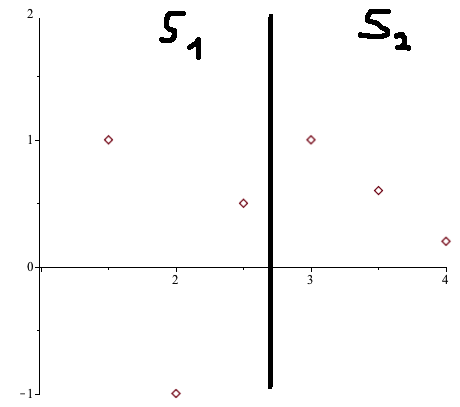
\includegraphics[width =\textwidth]{logos/PlotsBetter01.png}
			\end{minipage}
			\begin{minipage}{0.45\textwidth}
				Rekursionsstufe 1: Divide		
			\end{minipage}
		\end{frame}

		\begin{frame}{Beispiel}
			\begin{minipage}{0.45\textwidth}
				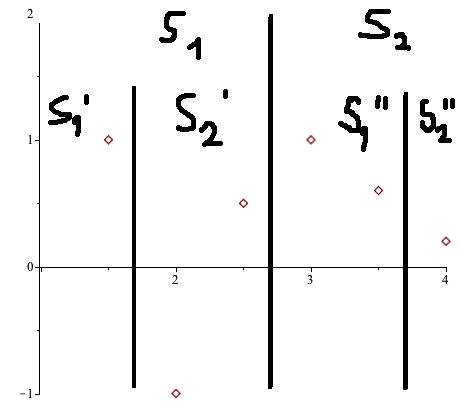
\includegraphics[width =\textwidth]{logos/PlotsBetter02.png}
			\end{minipage}
			\begin{minipage}{0.45\textwidth}
				Rekursionsstufe 2: Divide\\
				$S_1'  \text{ : }  \infty$ \\	
				$S_2'  \text{ : }  2.5 $ \\
				$S_1''  \text{ : }  0.41$ \\
				$S_2''  \text{ : }  \infty$		
			\end{minipage}
		\end{frame}

		\begin{frame}{Beispiel}
			\begin{minipage}{0.45\textwidth}
				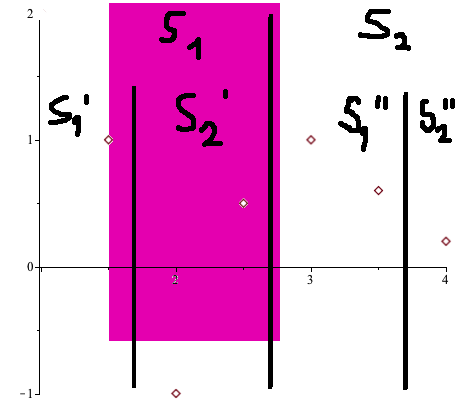
\includegraphics[width =\textwidth]{logos/PlotsBetter0gg.png}
			\end{minipage}
			\begin{minipage}{0.45\textwidth}
				\textbf{Pinkes Rechteck}\\
				Höhe: $ 2 * \min(\infty, 1.68)$\\ Breite: $ \min(\infty, 1.68) $\\
				\ \\
				$d_1' \text{ : }  \infty \\
				d_2'  \text{ : }  1.68 \\
				d_3'  \text{ : }  1.68$ \\ 
				\ \\
				$S_1 \text{ : } \min(\infty, 1.68, 1.68) = 1.68$
			\end{minipage}
		\end{frame}

		\begin{frame}{Beispiel}
			\begin{minipage}{0.45\textwidth}
				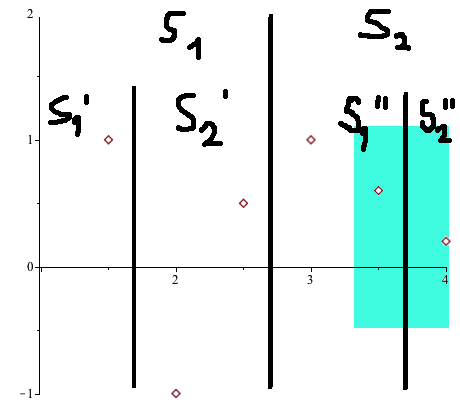
\includegraphics[width =\textwidth]{logos/PlotsBetter0g.png}
			\end{minipage}
			\begin{minipage}{0.45\textwidth}
				\textbf{Türkises Rechteck}\\
				Höhe: $ 2 * \min(0.64, \infty)$\\ Breite: $2 * \min(0.64, \infty) $\\
				\ \\
				$d_1'‘ \text{ : }  0.64 \\
				d_2'‘  \text{ : }  \infty \\
				d_3'‘  \text{ : }  0.64$ \\ 
				\ \\
				$S_2 \text{ : } \min(0.64, \infty, 0.64) = 0.64$
			\end{minipage}
		\end{frame}

		\begin{frame}{Beispiel}
			\begin{minipage}{0.45\textwidth}
				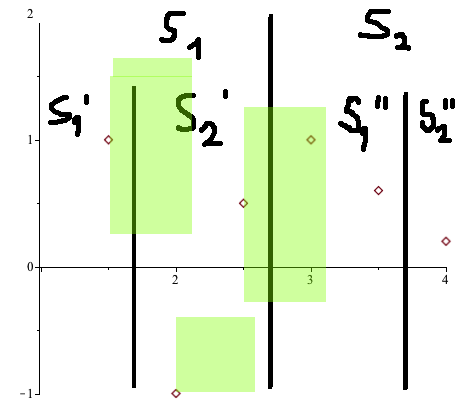
\includegraphics[width =\textwidth]{logos/PlotsBetter0ggg.png}
			\end{minipage}
			\begin{minipage}{0.45\textwidth}
				\textbf{Rechtecke}\\
				Höhe: $ 2 * \min(1.64, 0.64)$\\ Breite: $2 * \min(1.64, 0.64) $\\
				\ \\
				$d_1'‘ \text{ : }  1.64 \\
				d_2'‘  \text{ : }  0.64 \\
				d_3'‘  \text{ : }  0.707$ \\ 
				\ \\
				$\text{Gesamt  : } \min(1.64, 0.64, 0.707) = 0.64$

				Closest Pair ist $p_5$ und $p_6$ \\ mit Abstand $0.64$
			\end{minipage}
		\end{frame}






\end{document}
